\documentclass[lualatex, aspectratio=169]{beamer}

\usetheme{Data61}

\title{Aboleth}
\subtitle{Bayesian Neural Networks and More}
\author{Dan Steinberg}
\date{April 11, 2018}
\institute{Inference Systems Engineering}

\usepackage{fontspec}
\usepackage{color}
\usepackage{unicode-math}
\usefonttheme{serif}

\defaultfontfeatures{Ligatures=TeX}
\setmainfont{Open Sans}
\setsansfont{Open Sans}
\setmonofont{Inconsolata}
% \setmathfont{DejaVu Math Tex Gyre}
% \setmathfont{XITS Math}

% Math
\renewcommand{\v}[1]{\mathbf{#1}}
\renewcommand{\d}{\,\mathrm{d}}
\newcommand{\T}{^\top}
\newcommand{\vp}[1]{\mathbf{#1}^{\prime}}
\newcommand{\h}[1]{\hat{#1}}
\newcommand{\cov}[2]{\mathrm{Cov}(#1,#2)}
\newcommand{\hil}{\mathscr{H}}
\newcommand{\reals}{\mathbb{R}}
\newcommand{\complexs}{\mathbb{C}}
\newcommand{\dprod}[2]{{\langle #1, #2 \rangle}}
\newcommand{\expec}[1]{\mathbb{E}\!\left[{#1}\right]}
\newcommand{\argmin}{\operatornamewithlimits{argmin}}
\newcommand{\pd}[2]{\frac{\partial#1}{\partial#2}}
\newcommand{\norm}[1]{\|#1\|}
\newcommand{\query}[1]{{#1}^{*}}


% Text
\newcommand{\imp}[1]{\textcolor{Data61 green}{\textbf{#1}}}

%%%%%%%%%%%%%%%%%%%%%%%
% global renew commands
%%%%%%%%%%%%%%%%%%%%%%%
\makeatletter
\def\gnewcommand{\g@star@or@long\new@command}
\def\grenewcommand{\g@star@or@long\renew@command}
\def\g@star@or@long#1{% 
  \@ifstar{\let\l@ngrel@x\global#1}{\def\l@ngrel@x{\long\global}#1}}
\makeatother
%%%%%%%%%%%%%%%%%%%%%%%%%%%
% end global renew commands
%%%%%%%%%%%%%%%%%%%%%%%%%%%

\let\oldint\int
\grenewcommand\int{\oldint\!}
\grenewcommand{\epsilon}{\varepsilon}

\let\oldemptyset\emptyset
\let\emptyset\varnothing

\newtheorem{prp}{Proposition}[section]
\newtheorem{thm}{Theorem}[section]

\theoremstyle{definition}
\newtheorem{dfn}{Definition}[section]

\newcommand{\sidenote}[1]{
  \marginline{{\fontsize{8}{8}\selectfont
    \begin{spacing}{1}
#1
    \end{spacing} }}
}



\begin{document}

\maketitle

\begin{frame}{Outline}
  \begin{itemize}
    \item Supervised learning
    \item ...
  \end{itemize}
\end{frame}


\section{Supervised Learning \\ to Bayesian NNs}


\begin{frame}{Supervised learning}
  \begin{itemize}
    \item <1-> $\v{x}$ is a vector of covariates or features, $y$ a target 
    \item <2-> There exists an unknown function, $f$, that maps the covariates to the targets,
      \begin{align*}
        y = f(\v{x}) + \epsilon
      \end{align*}
    \item <3-> \emph{Supervised ML}: learn an approximation of this function, $h$, using examples,
      \begin{align*}
        y_i \approx h(\v{x}_i) \quad \text{for all} \quad \{(y_1, \v{x}_1), (y_2, \v{x}_2), \ldots,
          (y_N, \v{x}_N) \}
      \end{align*}
  \end{itemize}
\end{frame}


\begin{frame}{Supervised learning}
  Usually we parameterise $h$ by $\theta$, and learning is often \imp{optimisation} of these parameters,
  \begin{align*}
    \hat{\theta} = \argmin_\theta \frac{1}{N} \sum^N_{i=1} \mathcal{L}\!\left(y_i, h(\v{x}_i, \theta)\right),
  \end{align*}
  where $\mathcal{L}$ is a \imp{loss} or \imp{error} function.
  % For example, linear regression,
  % \begin{align*}
  %   \argmin_{\v{w}} \frac{1}{N} \sum^N_{i=1} \|y_i - \v{w}^\top \v{x}_i \|^2_2
  % \end{align*}

\end{frame}


\begin{frame}{Prediction}
  Once we have learned $h$, we want to use it to \imp{predict} $\query{y}$ for \imp{new}, \imp{unseen} instances of $\query{\v{x}}$,
  \begin{align*}
    \expec{\query{y}} = h(\query{\v{x}}, \hat{\theta}).
  \end{align*}
  with as little \imp{error} as possible --- we want $h$ to \imp{generalise} from example!
\end{frame}


\begin{frame}{Regression example}

  \begin{description}
    \item[True function] $f(x) = \sin(x)$
    \item[Observations] $y_i = f(x_i) + \epsilon_i, \quad \epsilon_i \sim \mathcal{N}(0, 0.1)$
  \end{description}

  \begin{figure}
    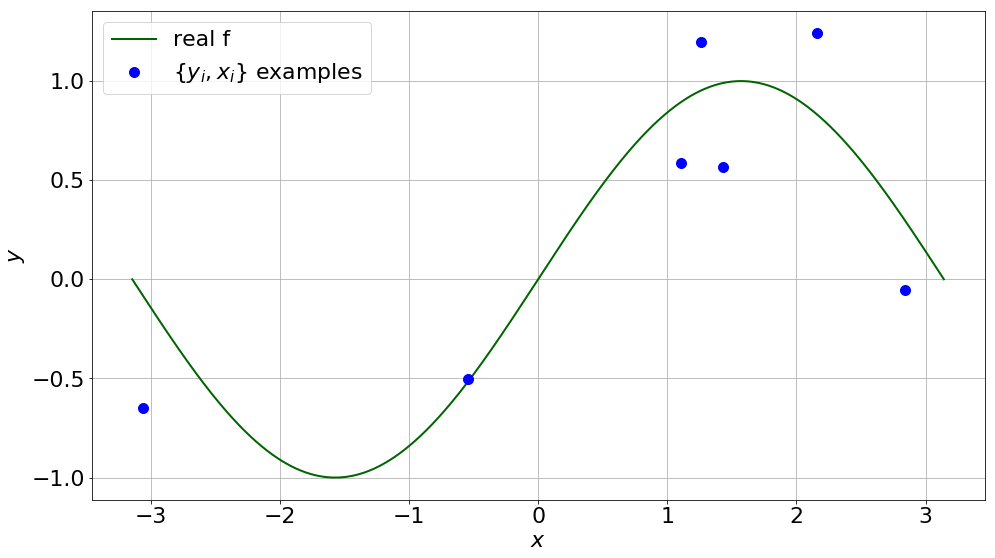
\includegraphics[width=0.5\pagewidth]{assets/regress.png}
  \end{figure}

\end{frame}


% \begin{frame}{Fit a line}

%   \begin{description}
%     \item[Model] $h(x) = w_0 + w_1 x$
%     \item[Objective] $\argmin_{\v{w}} \frac{1}{N} \sum^N_{i=1} \|y_i - h(x_i)\|^2_2$ 
%   \end{description}

%   \begin{figure}
%     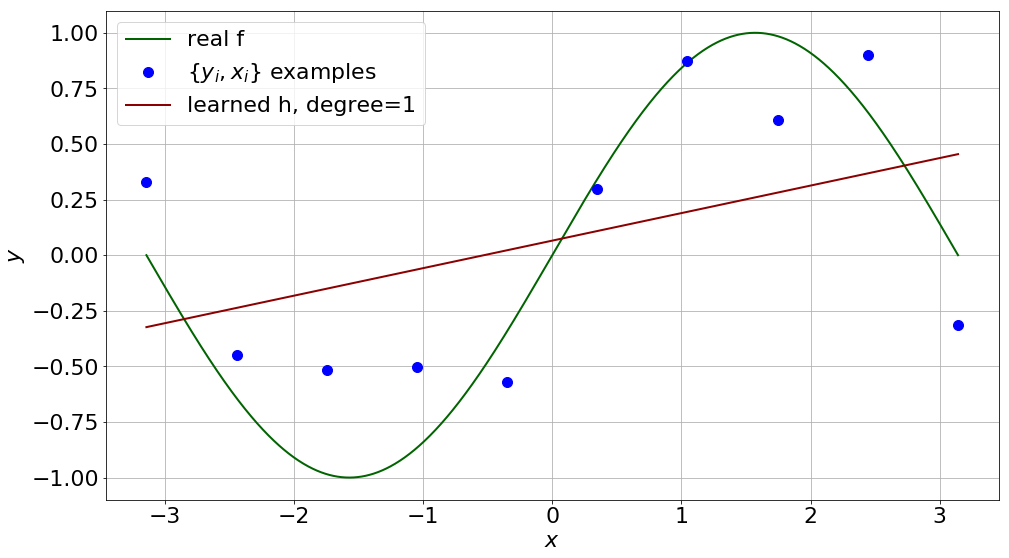
\includegraphics[width=0.5\pagewidth]{assets/poly1.png}
%   \end{figure}

%   Under-fitting --- bad generalisation/interpolation.

% \end{frame}


\begin{frame}{Fit a degree-3 polynomial}

  \begin{description}
    \item[Model] $h(x, \v{w}) = w_0 + w_1 x + w_2 x^2 + w_3 x^3$
    \item[Objective] $\argmin_{\v{w}} \frac{1}{N} \sum^N_{i=1} \|y_i - h(x_i, \v{w})\|^2_2$ 
  \end{description}

  \begin{figure}
    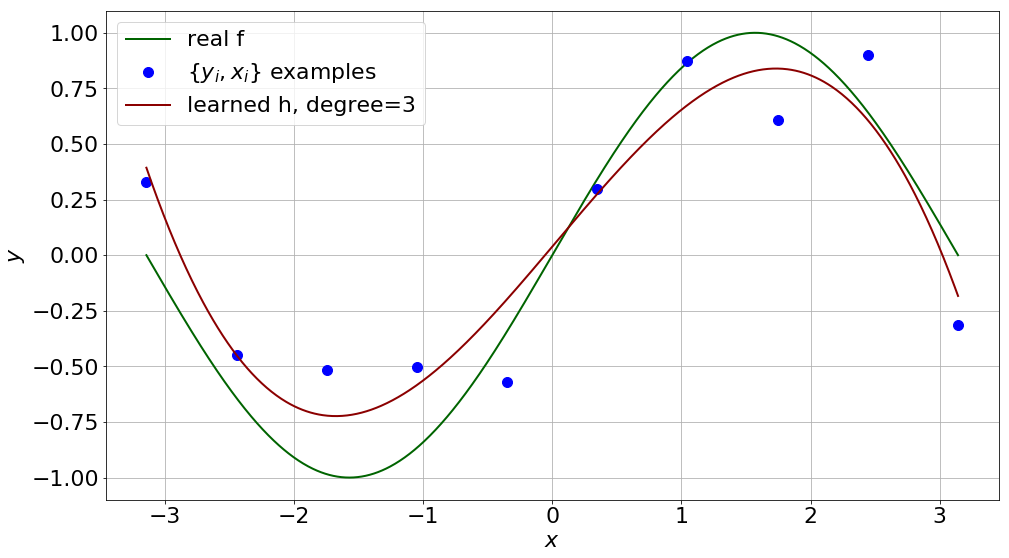
\includegraphics[width=0.5\pagewidth]{assets/poly3.png}
  \end{figure}

  Good fit --- good interpolation.

\end{frame}


\begin{frame}{Linear Models}

  So we saw a polynomial is one class of model, e.g.:
  \begin{align*}
    h(x, \v{w}) &= w_0 + w_1 x + w_2 x^2 + w_3 x^3 \\
                &= \begin{bmatrix} w_0 & w_1 & w_2 & w_3 \end{bmatrix}
                   \begin{bmatrix} 1 \\ x \\ x^2 \\ x^3 \end{bmatrix} \\
                   &= \v{w}\T \text{Poly}_3(x)
  \end{align*}
  This is part of a general class of models we call \imp{linear} models,
  \begin{align*}
    h(\v{x}, \v{w}) &= \v{w}\T \phi(\v{x})
  \end{align*}
  where $\phi$ is some function.

\end{frame}


\begin{frame}{Neural Nets}
  
  Neural nets generalise this class of linear models with \imp{non-linearities} ($\sigma$) and \imp{function composition}:
  \begin{itemize}
    \item 0 hidden layers: $\text{NN}_0(\v{x}) = \sigma_0( \v{W}_0\v{x} )$
    \item 1 hidden layer: $\text{NN}_1(\v{x}) = \sigma_1(\v{W}_1 \sigma_0( \v{W}_0 \v{x} ))$
    \item L hidden layers: $\text{NN}_L(\v{x}) = \sigma_L(\v{W}_L \sigma_{L-1}(\v{W}_{L-1} \ldots \sigma( \v{W}_0 \v{x} )))$
  \end{itemize}

  \begin{figure}
    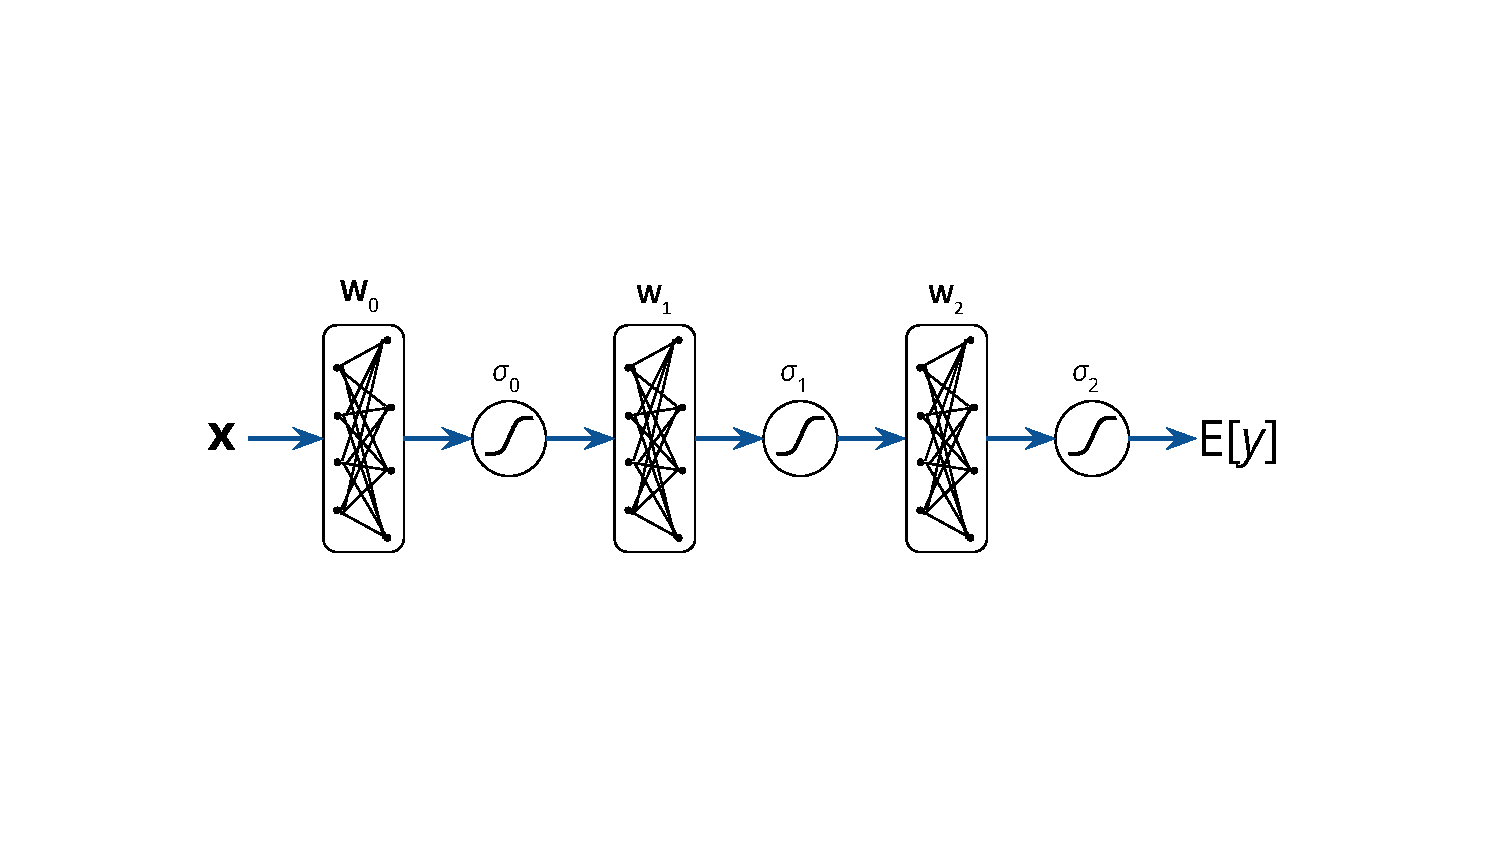
\includegraphics[page=1, trim={3cm 4.5cm 3.5cm 4.5cm}, clip, width=0.5\pagewidth]{assets/pictures.pdf}
  \end{figure}
  
\end{frame}


\begin{frame}{Why this representation?}

  \begin{itemize}
    \item Neural nets can represent any function!
    \item For a given depth, the more complex the function, the `wider' the layers have to be.
    \item Or we can use (exponentially) `narrower' and deeper nets!
  \end{itemize}

  Nice demo: \href{https://playground.tensorflow.org}{TensorFlow Playground}
  \begin{figure}
    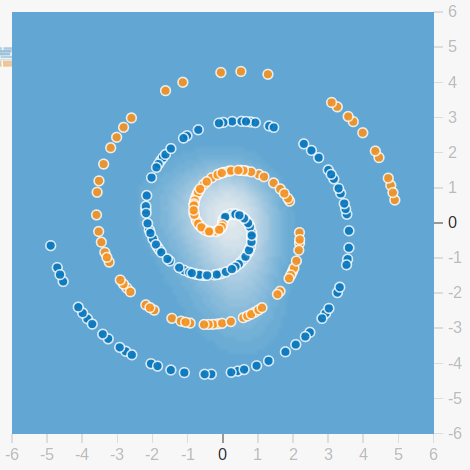
\includegraphics[width=0.2\pagewidth]{assets/swirl.png}
  \end{figure}


\end{frame}


\begin{frame}{TensorFlow Playground --- Spiral}

  \begin{figure}
    \centering
    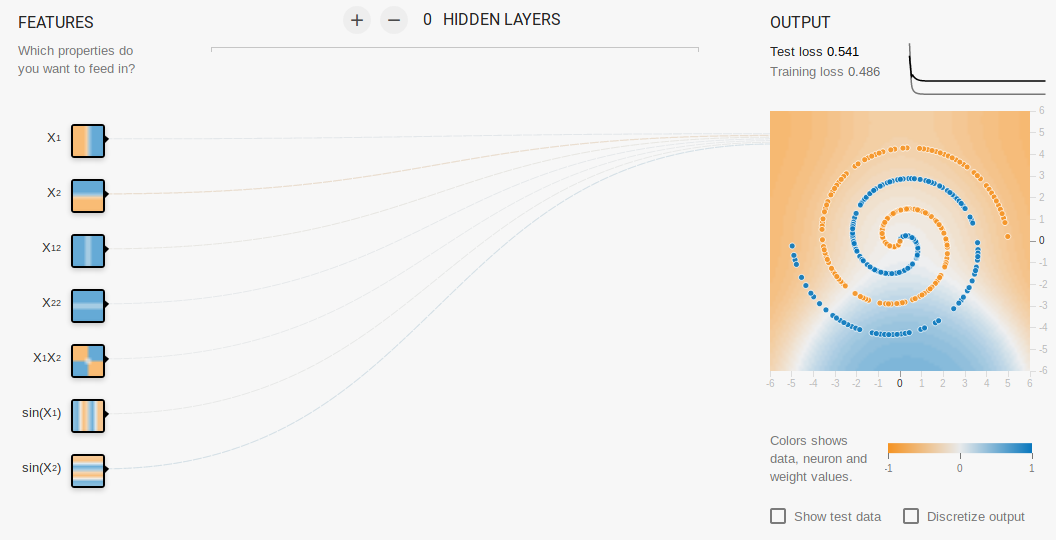
\includegraphics[height=0.75\pageheight]{assets/0-hidden.png}
  \end{figure}

\end{frame}


\begin{frame}{TensorFlow Playground --- Spiral}

  \begin{figure}
    \centering
    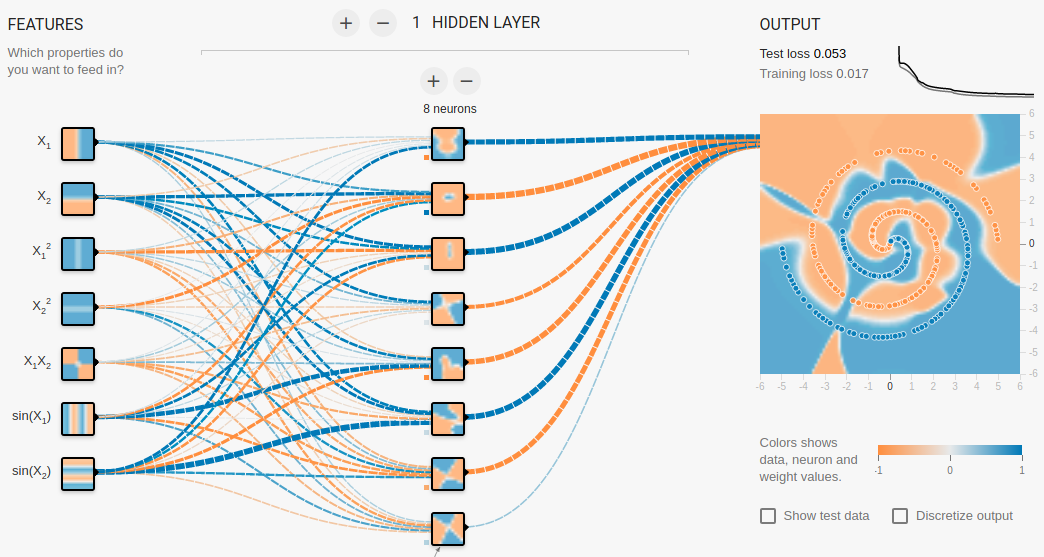
\includegraphics[height=0.75\pageheight]{assets/1-hidden.png}
  \end{figure}

\end{frame}


\begin{frame}{TensorFlow Playground --- Spiral}

  \begin{figure}
    \centering
    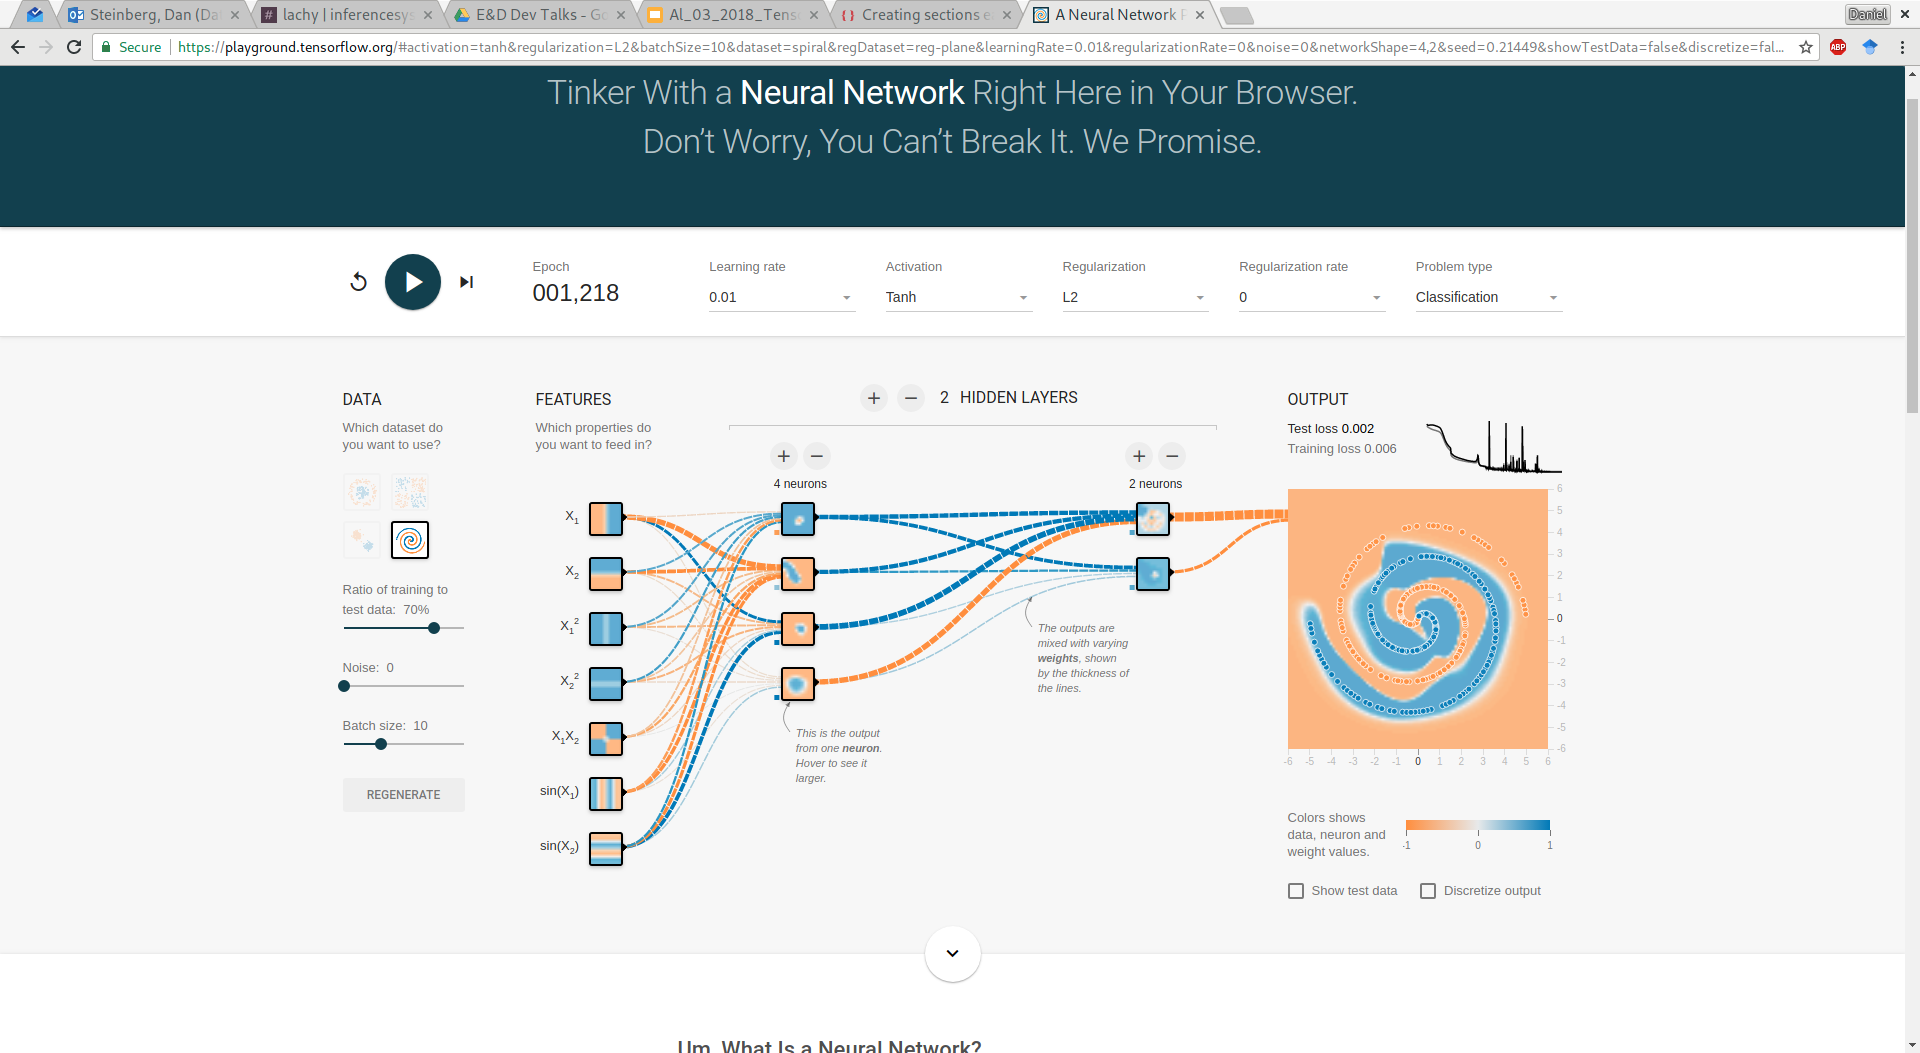
\includegraphics[height=0.75\pageheight]{assets/2-hidden.png}
  \end{figure}

\end{frame}


\begin{frame}{TensorFlow Playground --- Spiral}

  \begin{figure}
    \centering
    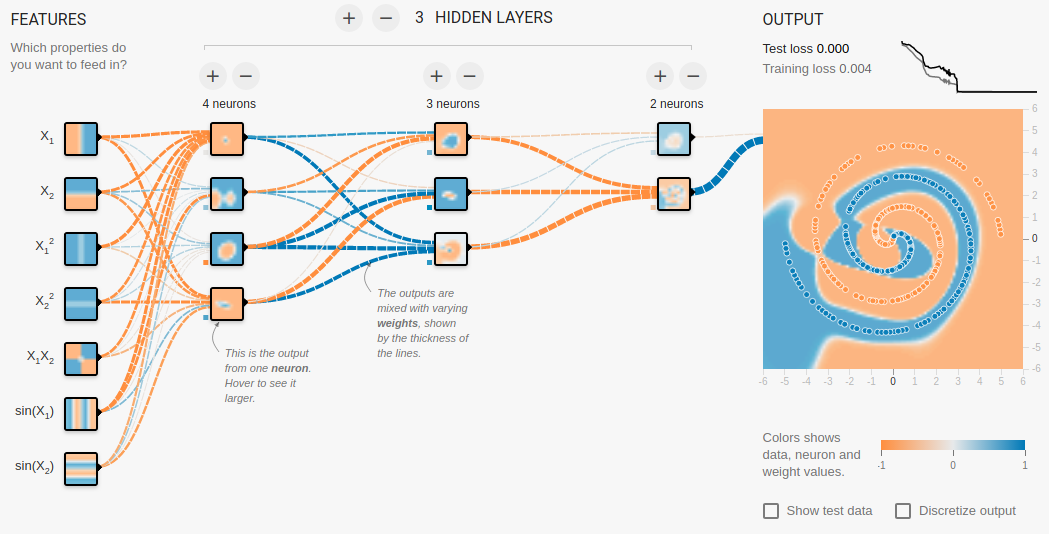
\includegraphics[height=0.75\pageheight]{assets/3-hidden.png}
  \end{figure}

\end{frame}


\begin{frame}{Neural Nets and Abstraction}

  \begin{figure}
    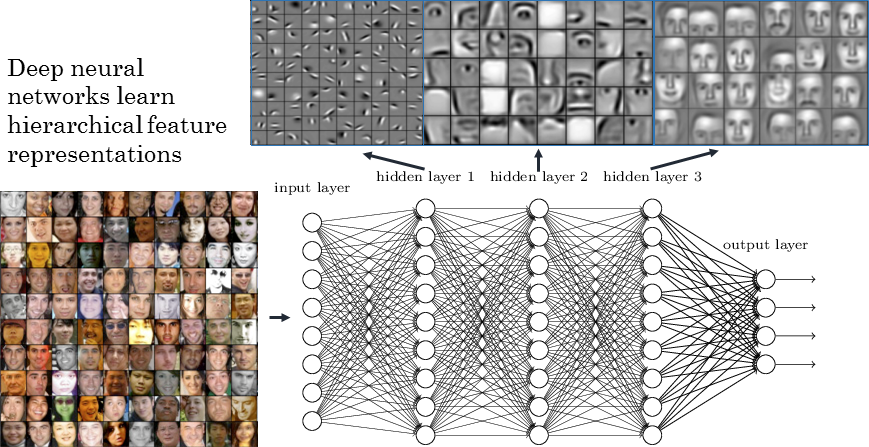
\includegraphics[width=0.7\pagewidth]{assets/abstraction.png}
    \caption{https://www.rsipvision.com/exploring-deep-learning/}
  \end{figure}

\end{frame}

% \begin{frame}{Fit a Degree-9 Polynomial}

%   \begin{description}
%     \item[Model] $h(x) = w_0 + w_1 x + \ldots + w_9 x^9$
%     \item[Objective] $\argmin_{\v{w}} \frac{1}{N} \sum^N_{i=1} \|y_i - h(x_i)\|^2_2$ 
%   \end{description}

%   \begin{figure}
%     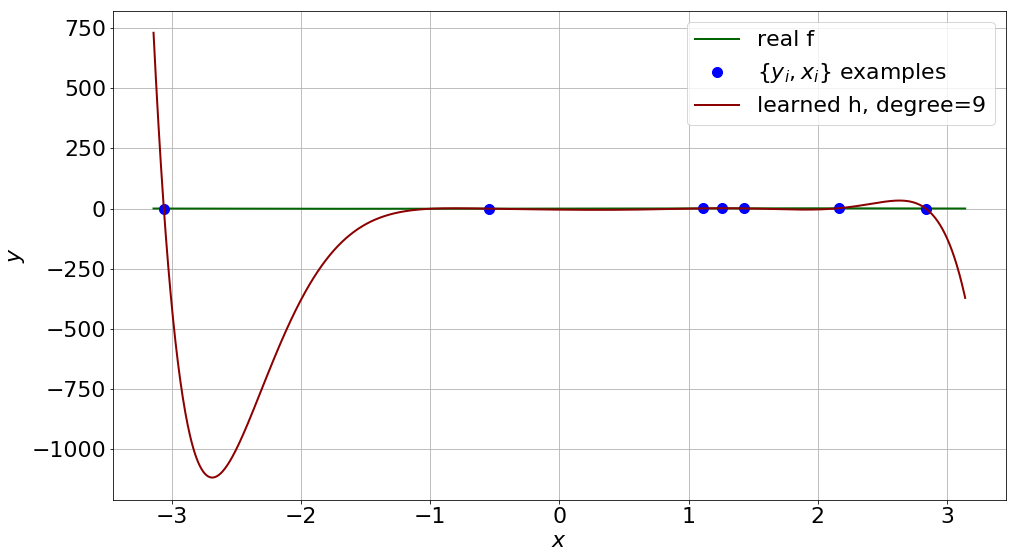
\includegraphics[width=0.5\pagewidth]{assets/poly9.png}
%   \end{figure}

%   Over fitting --- fits points exactly, but bad for interpolation.
% \end{frame}


% \begin{frame}{Regularisation}
%   TODO: why regularisation is important

%   TODO: what the learning objective looks like with regularisation
% \end{frame}


\begin{frame}{Probabilistic Prediction}
  TODO: We don't want just the expected value $\expec{\query{y} | \query{\v{x}}, \theta}$, but the predictive density, $p(\query{y} | \query{\v{x}}, \theta)$


  This still gives us an objective that is decomposable into data-fitting and regularisation...
\end{frame}


\begin{frame}{Bayesian Neural Nets}

  Probabilistic/Bayesian Neural networks

  Have to pass samples of the parameters through the network

  This is something that many existing frameworks do not do ... and it is something that has
  to be build into the graph!

\end{frame}


\section{Aboleth --- Features and design}


\begin{frame}{Features}
  TODO
\end{frame}


\begin{frame}{Why do we need another NN framework?}

  Why TensorFlow (and not PyTorch, Theano, MXNet)

  Why Not Keras, TensorFlow.learn, Edward, Zhusuan

\end{frame}


\begin{frame}{Design}
  TODO
\end{frame}


\begin{frame}{Applications}
  TODO  
\end{frame}



\end{document}
